\begin{frame}{Gradient Clipping}
    \begin{itemize}
        \item What will happen in case of a large gradient value?
        \pause
        \item The gradient descent will take us \textcolor{red}{far away} from our local position.
    \end{itemize}
	\begin{figure}[H]
		\centering
		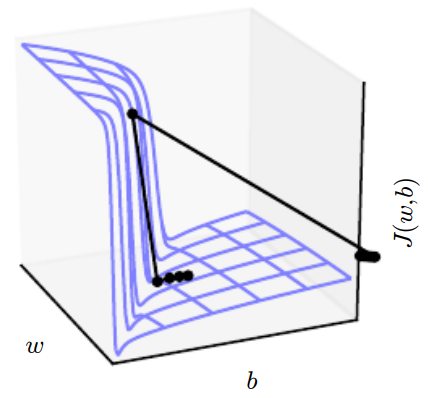
\includegraphics[width=0.4\textwidth]{Images/gard-clipping-1.png}
		\caption{The problem of large gradient value \cite{Goodfellow-et-al-2016}.}
	\end{figure}
\end{frame}

\begin{frame}{Gradient Clipping}
	\begin{itemize}
		\item Solve this problem simply by clipping gradient
		\item Two approaches to do so:
		\begin{itemize}
			\item Clipping by value
			\item Clipping by norm
		\end{itemize} 
	\end{itemize}
\end{frame}

\begin{frame}{Gradient Clipping by value}
	\begin{itemize}
		\item Set a max ($\alpha$) and min ($\beta$) threshold value
		\item For each index of gradient $\symbfit{g}_i$ if it is lower or greater than your threshold clip it:
		\begin{columns}
			\centering
			\begin{column}{0.45\textwidth}
				\centering
				\[
				\begin{aligned}
					&\text{if} \; \symbfit{g}_i > \alpha: \\
					&\qquad \symbfit{g}_i \gets \alpha \\
					&\text{else if} \; \symbfit{g}_i < \beta: \\
					&\qquad \symbfit{g}_i \gets \beta
				\end{aligned}
				\]
			\end{column}
			\begin{column}{0.45\textwidth}
				\centering
				\begin{figure}[H]
					\centering
					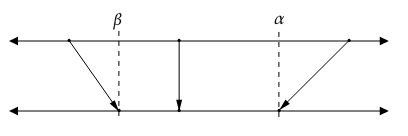
\includegraphics[width=0.95\textwidth]{Images/clipping-value.png}
				\end{figure}
			\end{column}
		\end{columns}
	\end{itemize}
\end{frame}

\begin{frame}{Gradient Clipping by value}
	\begin{figure}[H]
		\centering
		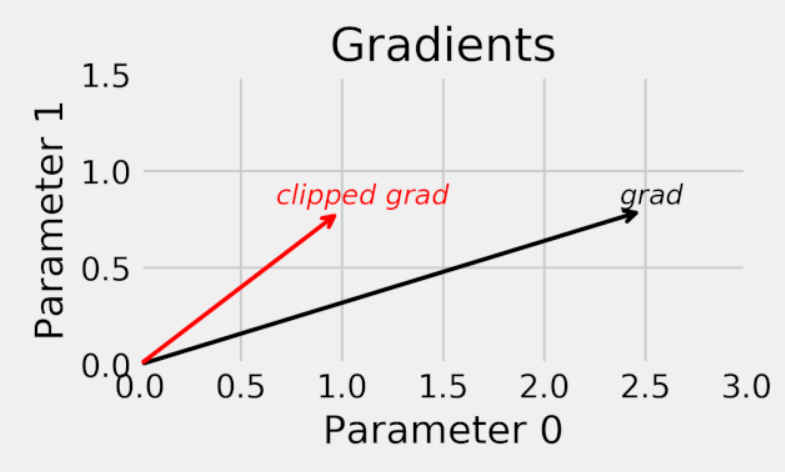
\includegraphics[width=0.5\textwidth]{Images/clip-by-value.png}
		\caption{The effect of clipping by value. \href{https://github.com/dvgodoy/PyTorchStepByStep/blob/master/ChapterExtra.ipynb}{source}}
	\end{figure}
	\begin{itemize}
		\item Clipping by value \textcolor{red}{will change gradient direction}.
		\item To preserve direction use clipping by norm.
	\end{itemize}
\end{frame}

\begin{frame}{Gradient Clipping by norm}
	\begin{itemize}
		\item Clip the norm $\|\symbfit{g}\|$ of the gradient $\symbfit{g}$ before updating parameters:
		\item[]
		\begin{columns}
			\centering
			\begin{column}{0.4\textwidth}
				\centering
				\[
				\begin{aligned}
					&\text{if} \; \|\symbfit{g}\| > v:\\
					&\qquad \symbfit{g} \gets \frac{\symbfit g}{\|\symbfit g\|} v
				\end{aligned}
				\]
			\end{column}
			\begin{column}{0.6\textwidth}
				\begin{figure}[H]
					\centering
					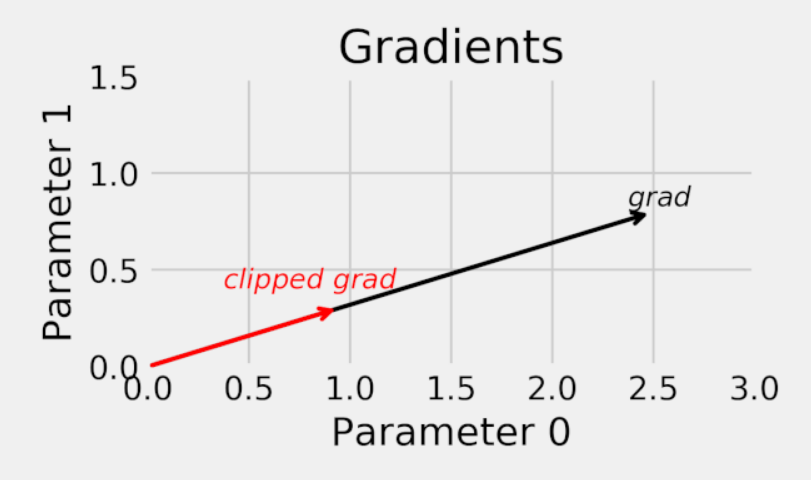
\includegraphics[width=0.5\textwidth]{Images/clip-by-norm.png}
					\caption{The effect of clipping by norm. \href{https://github.com/dvgodoy/PyTorchStepByStep/blob/master/ChapterExtra.ipynb}{source}}
				\end{figure}
			\end{column}
		\end{columns}
		
		$v$ is the threshold for clipping which is a hyperparameter.
		\item Gradient clipping saves the direction of gradient and controls its norm.
	\end{itemize}
\end{frame}

\begin{frame}{Gradient Clipping}
	\begin{itemize}
		\item There is one question, clipping by norm or value?
		\pause
		\item Clipping by value will not preserve the direction of the gradient, so it will send us to a bad neighborhood.
		\item Clipping by norm will preserve the direction and just control the value.
		\item So it is better to use clipping by \tc{keywords}{norm}.
	\end{itemize}
\end{frame}

\begin{frame}{Gradient Clipping}
	\begin{itemize}
		\item The effect of gradient clipping:
	\end{itemize}
	\begin{center}
		\begin{figure}[H]
			\centering
			\begin{minipage}{0.45\textwidth}
				\centering
				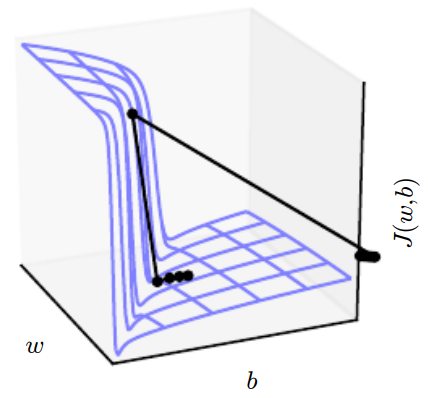
\includegraphics[width=0.8\textwidth]{Images/gard-clipping-1.png}
			\end{minipage}%\hfill
			\begin{minipage}{0.45\textwidth}
				\centering
				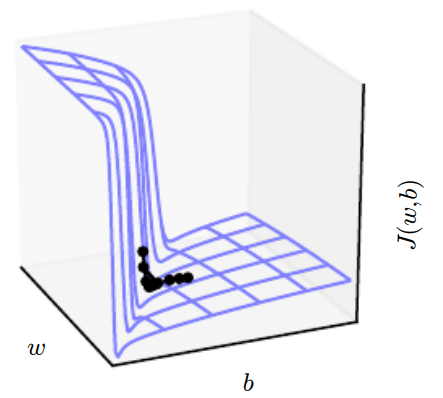
\includegraphics[width=0.8\textwidth]{Images/grad-clipping-2.png}
			\end{minipage}
			\caption{The "cliffs" landscape (left) without gradient clipping\\ and (right) with gradient clipping \cite{Goodfellow-et-al-2016}.}
		\end{figure}
	\end{center}
\end{frame}


%%%%%%%%%%%%%%%%%%%%%%%%%%%%%%%%%%%%%%%%%%%%%%%%%%%%%%%%%%%%%%%%%%%%%%%%%%%%%%%%%%
%%%%%%%%%%%%%%%%%%%%%%%%%%%%%%%%%%%%%%%%%%%%%%%%%%%%%%%%%%%%%%%%%%%%%%%%%%%%%%%%%%
\begin{frame}{Weight Initialization}
    \begin{itemize}
    	\item Is initialization really necessary?
    	\item What are the impacts of initialization?
    	\pause
%    	\item Weight initialization is critical for model performance.
    	\item A bad initialization may increase convergence time or even make optimization diverge.
    	\item How to initialize?
    	\begin{itemize}
    		\item Zero initialization
    		\item Random initialization
    	\end{itemize}
    \end{itemize}
	\begin{figure}[H]
		\centering
		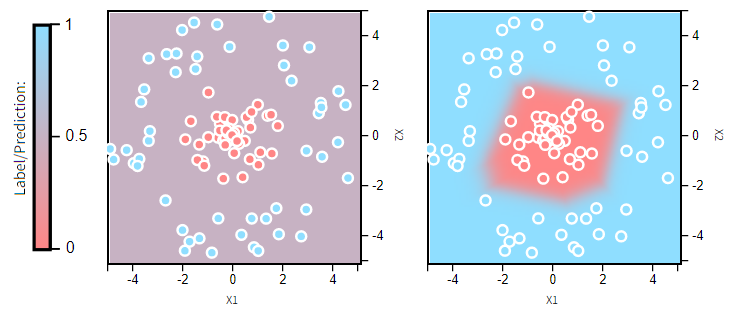
\includegraphics[width=0.65\textwidth]{Images/wi-crucial.png}
		\caption{The output of a three layer network after about 600 epoch. (left) using a bad\\ initialization method and (right) using an appropriate initialization \cite{katanforoosh-kunin}.}
	\end{figure}
\end{frame}

\begin{frame}{Weight Initialization}
	\begin{block}{Let's review some notations before we continue:}
		\begin{columns}
			\begin{column}{0.4\textwidth}
				\[
				\begin{cases}
					n^{[l]} := \text{layer $l$ neurons number}, \\
					W^{[l]} := \text{layer $l$ weights},\\
					b^{[l]} := \text{layer $l$ biases}, \\
					a^{[l]} := \text{layer $l$ outputs}
				\end{cases}
				\]
			\end{column}\hfill
			\begin{column}{0.4\textwidth}
				\begin{figure}[H]
					\centering
					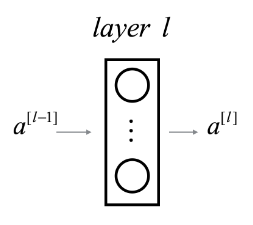
\includegraphics[width=0.65\textwidth]{Images/layer.png}
				\end{figure}
			\end{column}
		\end{columns}
	\end{block}
\end{frame}

\begin{frame}{Weight Initialization: Zero Initialization}
	\begin{block}{Zero Initialization method:}
		\[
		\begin{cases}
			W^{[l]} = \symbfit{0},\\
			b^{[l]} = \symbfit{0}
		\end{cases}
		\]
	\end{block}
	\begin{itemize}
		\item[]
		\item[]
		\item Simple but perform very poorly. (why?)
		\pause
		\item Zero initialization will lead each neuron to learn the same feature
		\item This problem is known as network {\color{red}failing to break symmetry}
		\item In fact any constant initialization suffers from this problem.
	\end{itemize}
\end{frame}

\begin{frame}{Weight Initialization: Zero Initialization}
	\begin{figure}[H]
		\centering
		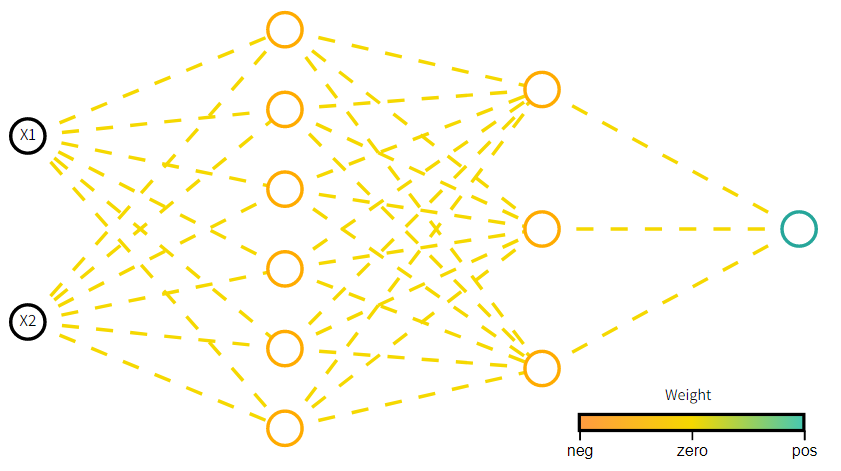
\includegraphics[width=0.65\textwidth]{Images/zero-init.png}
		\caption{As we can see network has failed to break symmetry. There has been no improvement in weights after about 600 epochs of training \cite{katanforoosh-kunin}.}
	\end{figure}
	\begin{itemize}
		\item[]
		\item We need to break symmetry. How? using randomness.
	\end{itemize}
\end{frame}

\begin{frame}{Weight Initialization: Random Initialization}
	\begin{itemize}
		\item To use randomness in our initialization we can use uniform or normal distribution:
		\medskip
		\item[]\begin{block}{General Uniform Initialization:}
			\[
			\begin{cases}
				W^{[l]} \sim U(-r, +r),\\
				b^{[l]} = 0
			\end{cases}
			\]
		\end{block}
		\item[]\begin{block}{General Normal Initialization:}
			\[
			\begin{cases}
				W^{[l]} \sim \mathcal{N}(\mu=0, \sigma^2),\\
				b^{[l]} = 0
			\end{cases}
			\]
		\end{block}
		\medskip
		\item But this is really crucial to choose $r$ or $\sigma$ properly.
	\end{itemize}
\end{frame}

%\begin{frame}{Weight Initialization: Random Initialization}
%	
%	\begin{block}{Simple Random Initialization:}
%		\[
%		\begin{cases}
%			W^{[l]} \sim \mathcal{N}\left(\mu=0, \sigma^2\right), \\
%			b^{[l]} = 0
%		\end{cases}
%		\]
%	\end{block}
%	\pause
%	\begin{itemize}
%		\item[]
%		\item[]
%		\item It depends on standard deviation ($\sigma$) value
%		\item If it choose carefully, will perform well for small networks
%		\item One can use $\sigma = 0.01$ as a best practice.
%		\item But still has problems with deeper networks.
%		\item Too small/large value for $\sigma$ will lead to vanishing/exploding gradient problem.
%	\end{itemize}
%\end{frame}

\begin{frame}{Weight Initialization: Random Initialization}
	\begin{figure}[H]
		\centering
		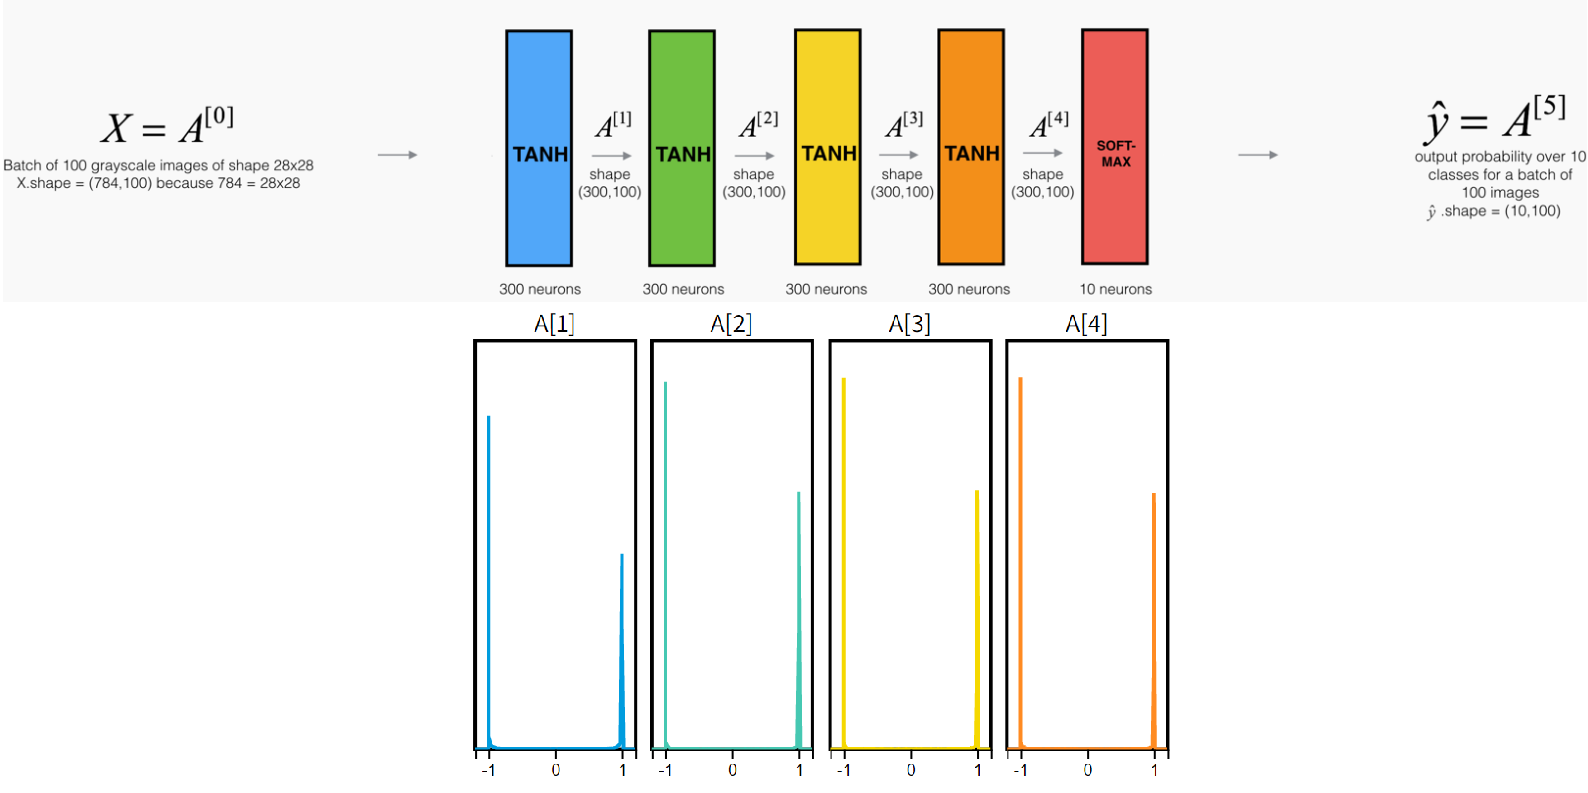
\includegraphics[width=0.9\textwidth]{Images/normal-init.png}
		\caption{Uniform initialization problem. On the top, you can see the model architecture, and on the bottom, you can see the density of each layer's output. Model has trained on MNIST dataset for 4 epoch. Weights are initialized randomly from $U(\frac{-1}{\sqrt{n^{[l-1]}}}, \frac{1}{\sqrt{n^{[l-1]}}})$ \cite{katanforoosh-kunin}.}
	\end{figure}
\end{frame}

\begin{frame}{Weight Initialization: Random Initialization}
	\begin{itemize}
		\item How to choose $r$ or $\sigma$?
		\item We need to follow these rules:
		\begin{itemize}
			\item keep the mean of the activations zero.
			\item keep the variance of the activations same across every layer.
		\end{itemize}
		\item How to do so?
	\end{itemize}
\end{frame}

\begin{frame}{Weight Initialization: Xavier Initialization}
	\begin{block}{Xavier Initialization:}
		\begin{itemize}
			\item For Uniform distribution use:
			\[
			r = \sqrt{\frac{3}{\text{fan}_\text{avg}}}
			\]
			
			\medskip
			\item For Normal distribution use:
			\[
				\sigma^2 = \frac{1}{\text{fan}_\text{avg}}
			\]
			\item Where:
			\[
			\text{fan}_\text{avg} = \frac{n^{[l-1]} + n^{[l]}}{2}
			\]
		\end{itemize}
		{\scriptsize (You can read about why this method works at \cite{katanforoosh-kunin}.)}
	\end{block}
	\begin{itemize}
		\medskip
		\medskip
		\item Xavier initialization works well on \tc{keywords}{Tanh, Logestic or Sigmoid} activation function.
	\end{itemize}
\end{frame}


\begin{frame}{Weight Initialization: Random Initialization}
	\begin{figure}[H]
		\centering
		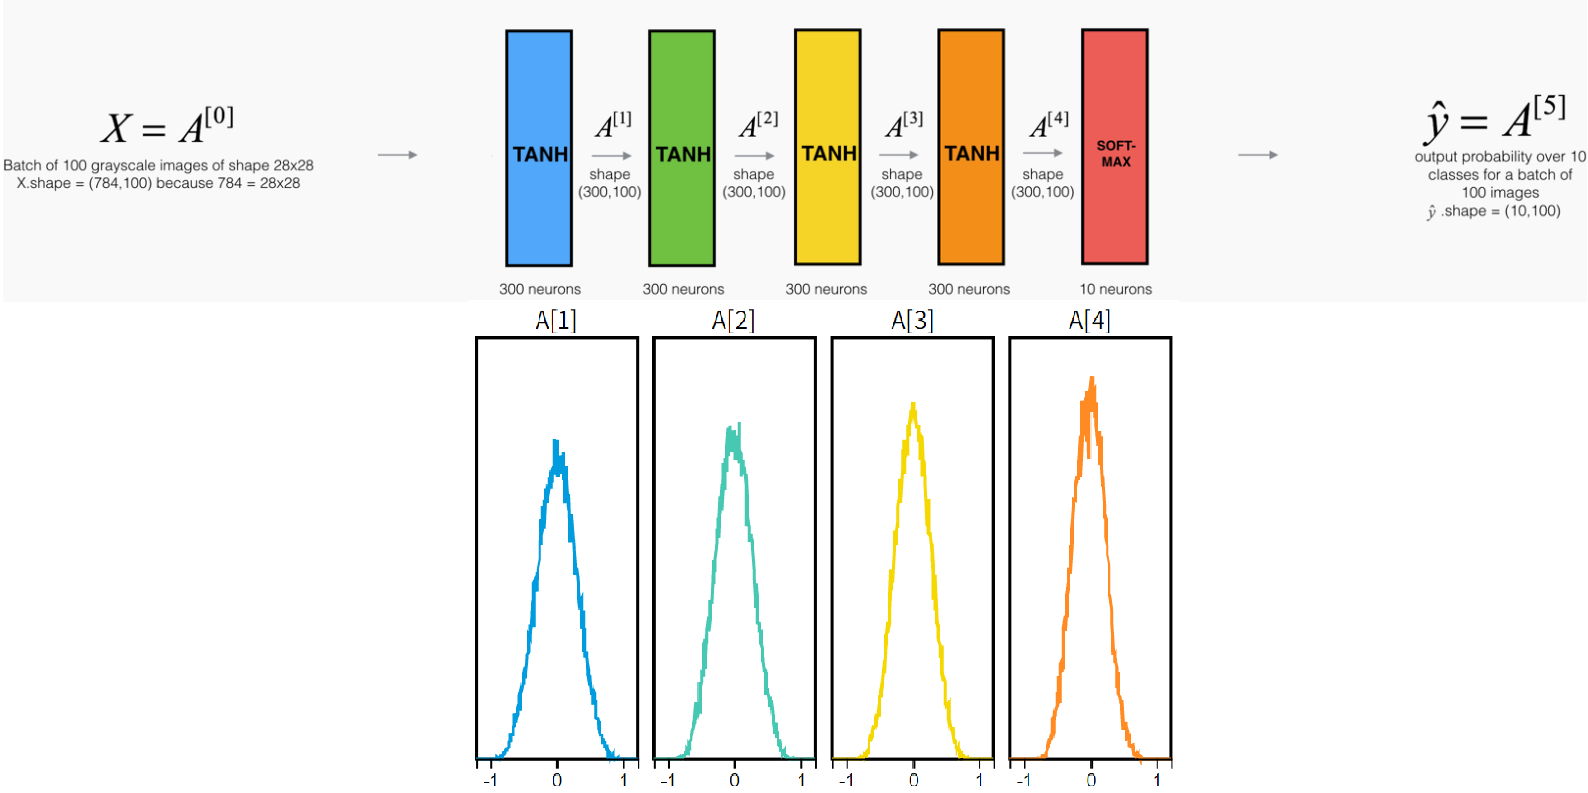
\includegraphics[width=0.9\textwidth]{Images/xavier-init.png}
		\caption{Vanishing gradient is no longer problem using Xavier initialization. Model has trained on MNIST dataset for 4 epoch. \cite{katanforoosh-kunin}.}
	\end{figure}
\end{frame}

\begin{frame}{Weight Initialization: He Initialization}
	\begin{itemize}
		\item Be careful that there is no universal method to choose $r$ and $\sigma$.
		\item Different method has proposed for different activation functions.
	\end{itemize}
	\begin{block}{He Initialization:}
		\begin{itemize}
			\item For Normal distribution:
			\[
			\sigma^2 = \frac{2}{n^{[l]}}
			\]
			\item For Uniform distribution:
			\[
			r = \sqrt{3\sigma^2}
			\]
		\end{itemize}
	\end{block}
	\begin{itemize}
		\medskip
		\medskip
		\item He initialization works well on \tc{keywords}{ReLU and its variants}.
	\end{itemize}
\end{frame}

\begin{frame}{Weight Initialization}
	\begin{itemize}
		\item So we talked about how to initialize weight
		\item Initializing well will solve problem of vanishing gradient problem.
		\item Different method have been proposed to initialize weights for different activation function.
		\item[]
		\item[]
		\item Use Xavier initialization for \tc{keywords}{Tanh, Logistic or Sigmoid} activation functions.
		\item Use He initialization for \tc{keywords}{ReLU and its variants}.
	\end{itemize}
\end{frame}

%\begin{frame}{Weight Initialization}
%	\begin{itemize}
%		\item We discussed weight initialization in previous slides.
%		\item A good initialization will help the model with the vanishing/exploding gradient problem.
%		\item Xavier method works well with $\tanh$ activation function.
%		\begin{itemize}
%			\item If you use $ReLU$ activation use He initialization:
%			\begin{block}{He Initialization:}
%				\setlength{\textwidth}{0.4\textwidth}
%				\[
%				\begin{cases}
%					W^{[l]} \sim \mathcal{N}\left(\mu=0, \sigma^2=\frac{2}{n^{[l]}}\right), \\
%					b^{[l]} = 0
%				\end{cases}
%				\]
%			\end{block}
%		\end{itemize}
%	\end{itemize}
%\end{frame}

%%%%%%%%%%%%%%%%%%%%%%%%%%%%%%%%%%%%%%%%%%%%%%%%%%%%%%%%%%%%%%%%%%%%%%%%%%%%%%%%%%
%%%%%%%%%%%%%%%%%%%%%%%%%%%%%%%%%%%%%%%%%%%%%%%%%%%%%%%%%%%%%%%%%%%%%%%%%%%%%%%%%%
\begin{frame}{Various GD types}
    \begin{itemize}
    	\item So far you got familiar with gradient-based optimization
    	\item If $\symbfit{g} = \nabla_{\symbfit{\theta}} \mathcal{J}$, then we will update parameters with this simple rule:
    	\[
    	\symbfit{\theta} \gets \symbfit{\theta} - \alpha\symbfit{g}
    	\]
    	\item[]
    	\item But there is one question here, how to compute $\symbfit{g}$?
    	\item Based on how we calculate $\symbfit{g}$ we will have different types of gradient descent:
    	\begin{itemize}
    		\item Batch Gradient Descent
    		\item Stochastic Gradient Descent
    		\item Mini-Batch Gradient Descent
    	\end{itemize}
    \end{itemize}
\end{frame}

\begin{frame}{Various GD types}
	\begin{block}{Review before continue:}
		Training cost function ($\mathcal{J}$) over a dataset usually is the average of loss function ($\mathcal{L}$) on entire training set, so for a dataset $\mathcal{D}=\{d_i\}_{i=1}^n$ we have:
		\[
		\mathcal{J}(\mathcal{D}) = \frac{1}{n} \sum_{i=1}^{n} \mathcal{L}(d_i; \symbfit{\theta})
		\] 
	\end{block}
\end{frame}

\begin{frame}{Various GD types: Batch Gradient Descent}
	\begin{itemize}
		\item In this type we use \tc{keywords}{entire training set} to calculate gradient
		\begin{block}{Batch Gradient:}
			\[
			\symbfit{g} = \frac{1}{n}\sum_{i=1}^n \nabla_{\symbfit{\theta}} \mathcal{L}(d_i, \symbfit{\theta})
			\]
		\end{block}
		\item[]
		\item This really needs huge computation and so is slow for large training sets.
	\end{itemize}
\end{frame}

\begin{frame}{Various GD types: Batch Gradient Descent}
	\begin{figure}[H]
		\centering
		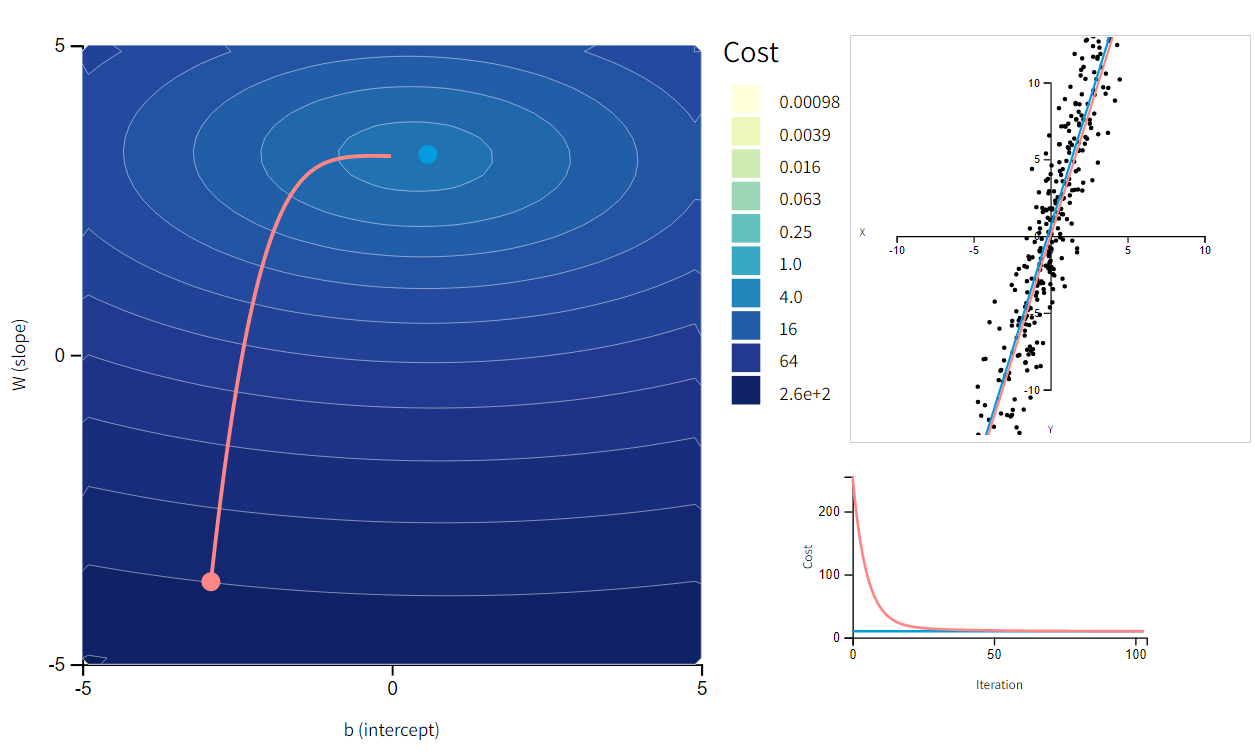
\includegraphics[width=0.8\textwidth]{Images/bgd.png}
		\caption{Optimization of parameters using BGD. Movement is very smooth \cite{katanforoosh-kunin-opt}.}
	\end{figure} 
\end{frame}

\begin{frame}{Various GD types: Stochastic Gradient Descent}
	\begin{itemize}
		\item Instead of calculating exact gradient, we can estimate it using our data
		\item This is exactly what SGD does, it estimates gradient using \tc{keywords}{only single data point}
		\begin{block}{Stochastic Gradient:}
			\[
			\hat{\symbfit{g}} = \nabla_{\symbfit{\theta}} \mathcal{L}(d_i, \symbfit{\theta})
			\]
		\end{block}
		\item[]
		\item As we use an approximation of gradient, instead of gently decreasing, the cost function will bounce up and down and decrease only on average.
		\item This method is really computationally efficient cause we only need to calculate gradient for one point per iteration. 
	\end{itemize}
\end{frame}

\begin{frame}{Various GD types: Stochastic Gradient Descent}
	\begin{figure}[H]
		\centering
		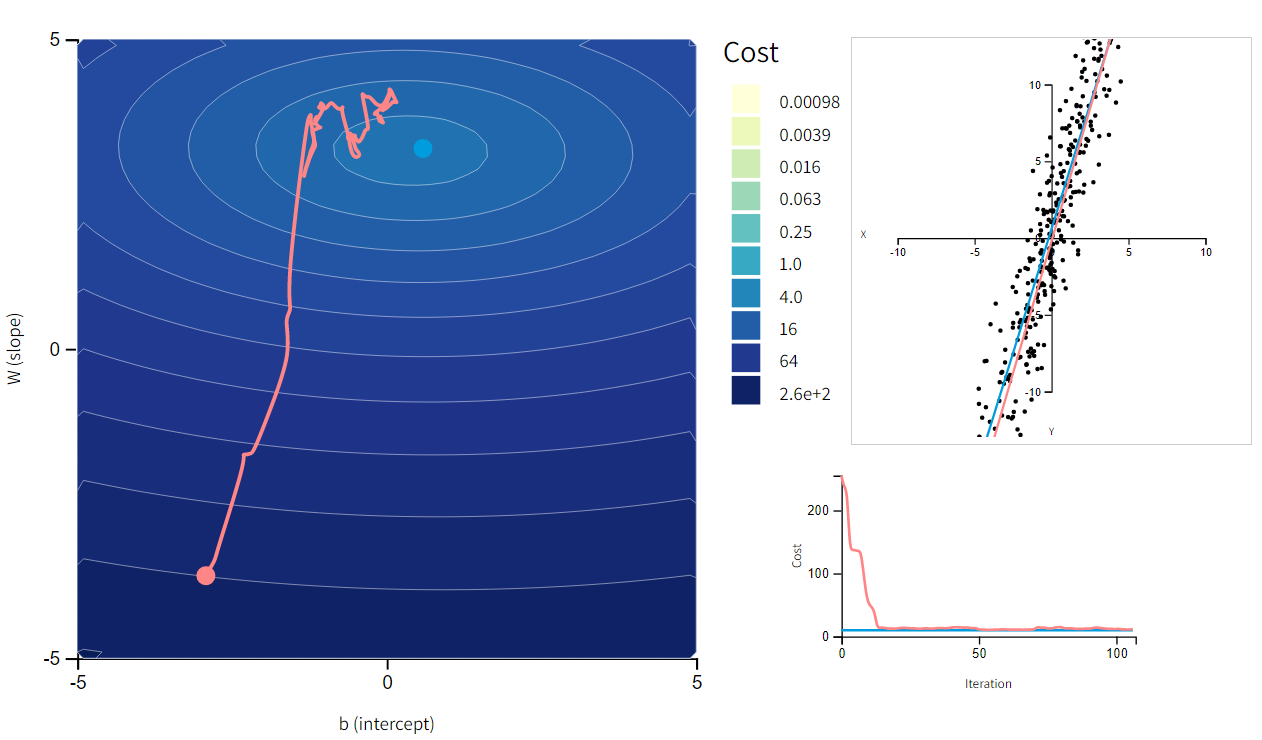
\includegraphics[width=0.8\textwidth]{Images/sgd.png}
		\caption{Optimization of parameters using SGD. As we expect, the movement is not that smooth \cite{katanforoosh-kunin-opt}.}
	\end{figure} 
\end{frame}

\begin{frame}{Various GD types: Mini-Batch Gradient Descent}
	\begin{itemize}
		\item In this method we still use estimation idea But use \tc{keywords}{a batch of data} instead of one point.
		\begin{block}{Mini-Batch Gradient:}
			\[
			\hat{\symbfit{g}} = \frac{1}{|\mathcal{B}|} \sum_{d\in\mathcal{B}} \nabla_{\symbfit{\theta}} \mathcal{L}(d, \symbfit{\theta}), \quad \mathcal{B} \subset \mathcal{D}
			\]
		\end{block}
		\item[]
		\item A better estimation than SGD
		\item With this way we can get a performance boost from hardware optimization, especially when using GPUs.
		\item Batch size ($|\mathcal{B}|$) is a hyperparameter you need to tune.
	\end{itemize}
\end{frame}

\begin{frame}{Various GD types: Mini-Batch Gradient Descent}
	\begin{figure}[H]
		\centering
		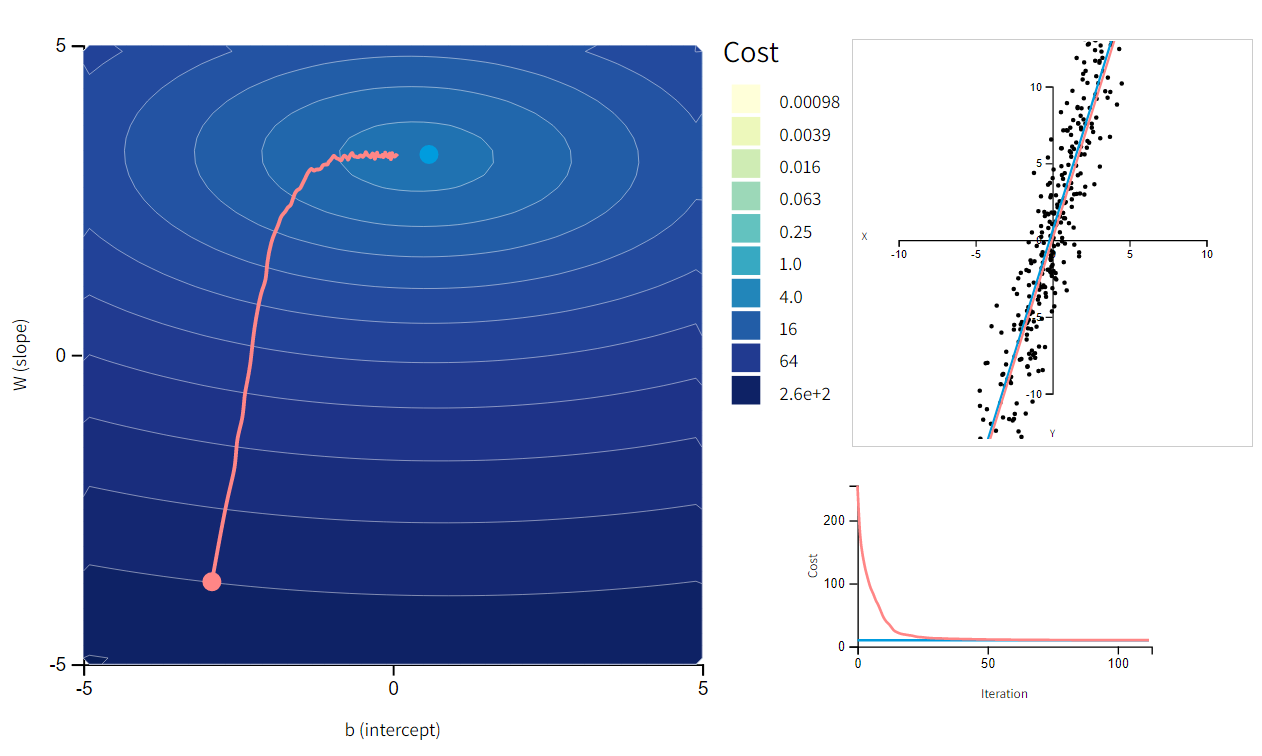
\includegraphics[width=0.8\textwidth]{Images/mbgd.png}
		\caption{Optimization of parameters using MBGD. The movement is much smother than SGD and behave like BGD \cite{katanforoosh-kunin-opt}.}
	\end{figure} 
\end{frame}

\begin{frame}{Various GD types}
	\begin{itemize}
		\item Now that we know what a batch is, we can define epoch and iteration:
		\begin{itemize}
			\item One \tc{keywords}{Epoch} is when an entire dataset is passed forward and backward through the network only once.
			\item One \tc{keywords}{Iteration} is when a batch is passed forward and backward through the network. 
		\end{itemize}
		
		\begin{figure}[H]
			\centering
			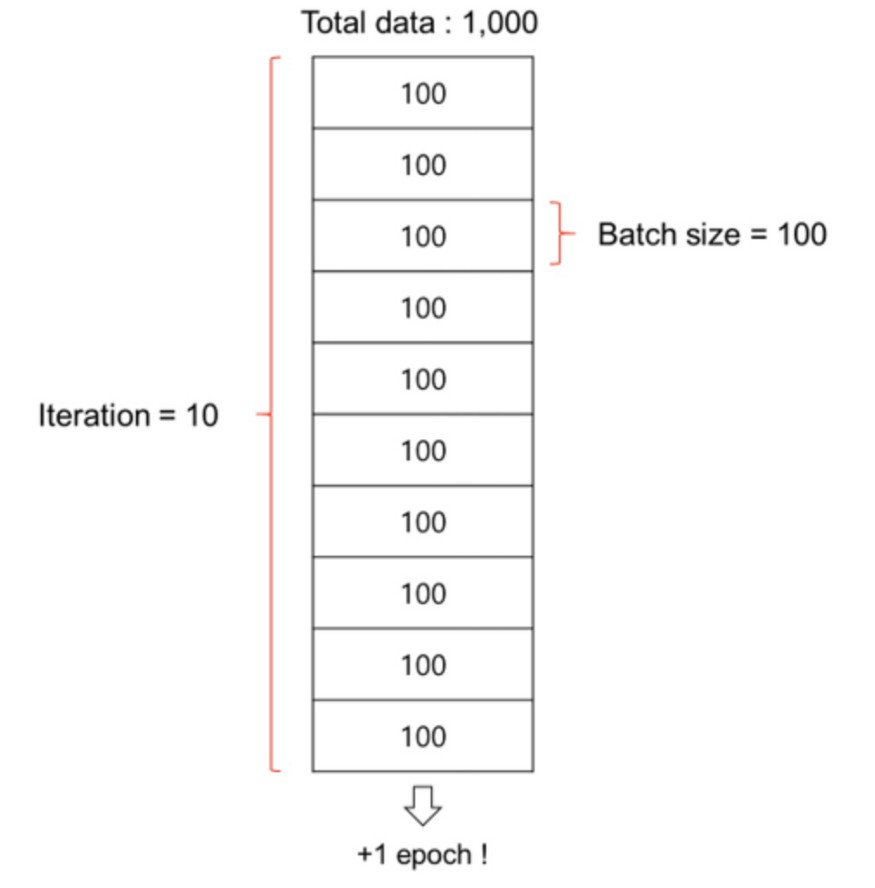
\includegraphics[width=0.4\textwidth]{Images/epoch-iteration.png}
			\caption{Epoch vs Iteration, \href{https://jerryan.medium.com/batch-size-a15958708a6}{source}.}
		\end{figure} 
	\end{itemize}
\end{frame}

\begin{frame}{Various GD types}
	\begin{itemize}
		\item So we got familiar with different types of GD.
		\begin{itemize}
			\item[\color{darkgreen}$\checkmark$] Batch Gradient Descent (BGD)
			\item[\color{darkgreen}$\checkmark$] Stochastic Gradient Descent (SGD)
			\item[\color{darkgreen}$\checkmark$] Mini-Batch Gradient Descent (MBGD)
		\end{itemize}
		\item[]
		\item[]
		\item The most recommended one is MBGD, because it is computational efficient.
		\item Choosing the right batch size is important to ensure convergence of the cost function and parameter values, and to the generalization of your model.
	\end{itemize}
\end{frame}